\usetikzlibrary{shadings}
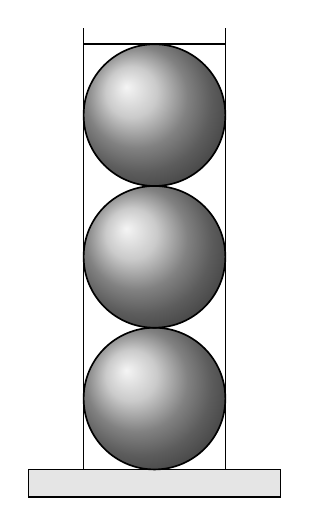
\begin{tikzpicture}[x=1cm,y=1cm,font=\normalsize]
% Cylindrical container with three tangent balls on a base platform.
% Walls tangent to balls; water line tangent to top ball; base top tangent to bottom ball.
\draw[line width=.6pt] (-0.9,0) -- (-0.9,5.6);
\draw[line width=.6pt] (0.9,0) -- (0.9,5.6);
\draw[line width=.6pt] (-0.9,5.4) -- (0.9,5.4);
\draw[line width=.6pt,fill=gray!20] (-1.6,-0.35) rectangle (1.6,0);
\shade[ball color=gray!55,draw=black,line width=.6pt] (0,0.9) circle (0.9);
\shade[ball color=gray!55,draw=black,line width=.6pt] (0,2.7) circle (0.9);
\shade[ball color=gray!55,draw=black,line width=.6pt] (0,4.5) circle (0.9);
\end{tikzpicture}
